\documentclass[pdftex,aspectratio=169]{beamer}

% Setup UTF-8 encoding
\usepackage[utf8]{inputenc}
\usepackage[T1]{fontenc}

%\usepackage{flashmovie}

% Setup beamer look theme
\mode<presentation>
{
	\useinnertheme{rectangles}
	\useoutertheme{infolines}
%	\usecolortheme{crane}
%	\usecolortheme{dove}
	\usecolortheme{seagull}
	\setbeamertemplate{navigation symbols}{}
}

% Use nicer font
\usepackage{palatino}
\usepackage{palatino,graphics,array}


% Setup czech language
\usepackage[czech]{babel}

% Include usefull packages
\usepackage{graphics}

% Include hyperlinks support
\usepackage{hyperref}
\hypersetup{colorlinks=true,linkcolor=black,urlcolor=black,unicode=true}

% Add support for simple URLs
\usepackage{url}

\usepackage{tikz}

\usepackage{verbatim}
\usetikzlibrary{arrows,shapes}
\usetikzlibrary{mindmap,trees}


% Commands for CC license
\newcommand{\CcLongnameByNcSa}{\href{http://creativecommons.org/licenses/by-nc-sa/3.0/cz/}{Attribution-Noncommercial-ShareAlike}}
\newcommand{\CcImageBy}[1]{
\includegraphics[scale=#1]{graphics/cc-by-white.pdf}}
\newcommand{\CcImageNc}[1]{
\includegraphics[scale=#1]{graphics/cc-nc-white.pdf}}
\newcommand{\CcImageSa}[1]{
\includegraphics[scale=#1]{graphics/cc-sa-white.pdf}}
\newcommand{\CcGroupByNcSa}[2]{\CcImageBy{#1}\hspace*{#2}\CcImageNc{#1}\hspace*{#2}\CcImageSa{#1}}




\title{Scheduling the GRID(s)}
\subtitle{an introduction to job scheduling in GRID environment}
\author[]{Mgr.~Šimon~Tóth}
\institute[FI@MU]{Faculty of Informatics @ Masaryk University}
\date{\today}

\newcommand{\CcNote}[1]{% longname
	Licensed under: \textit{Creative Commons #1 3.0 License}.%
}

\begin{document}

\pgfdeclarelayer{background}
\pgfsetlayers{background,main}

\begin{frame}
\titlepage
	\vfill
	\begin{center}
		\CcGroupByNcSa{0.33}{0.95ex}\\ {\tiny\CcNote{\CcLongnameByNcSa}}
		\vspace*{2ex}
	\end{center}
\end{frame}

\section{Introduction}
\subsection{Computing models}

{
\usebackgroundtemplate{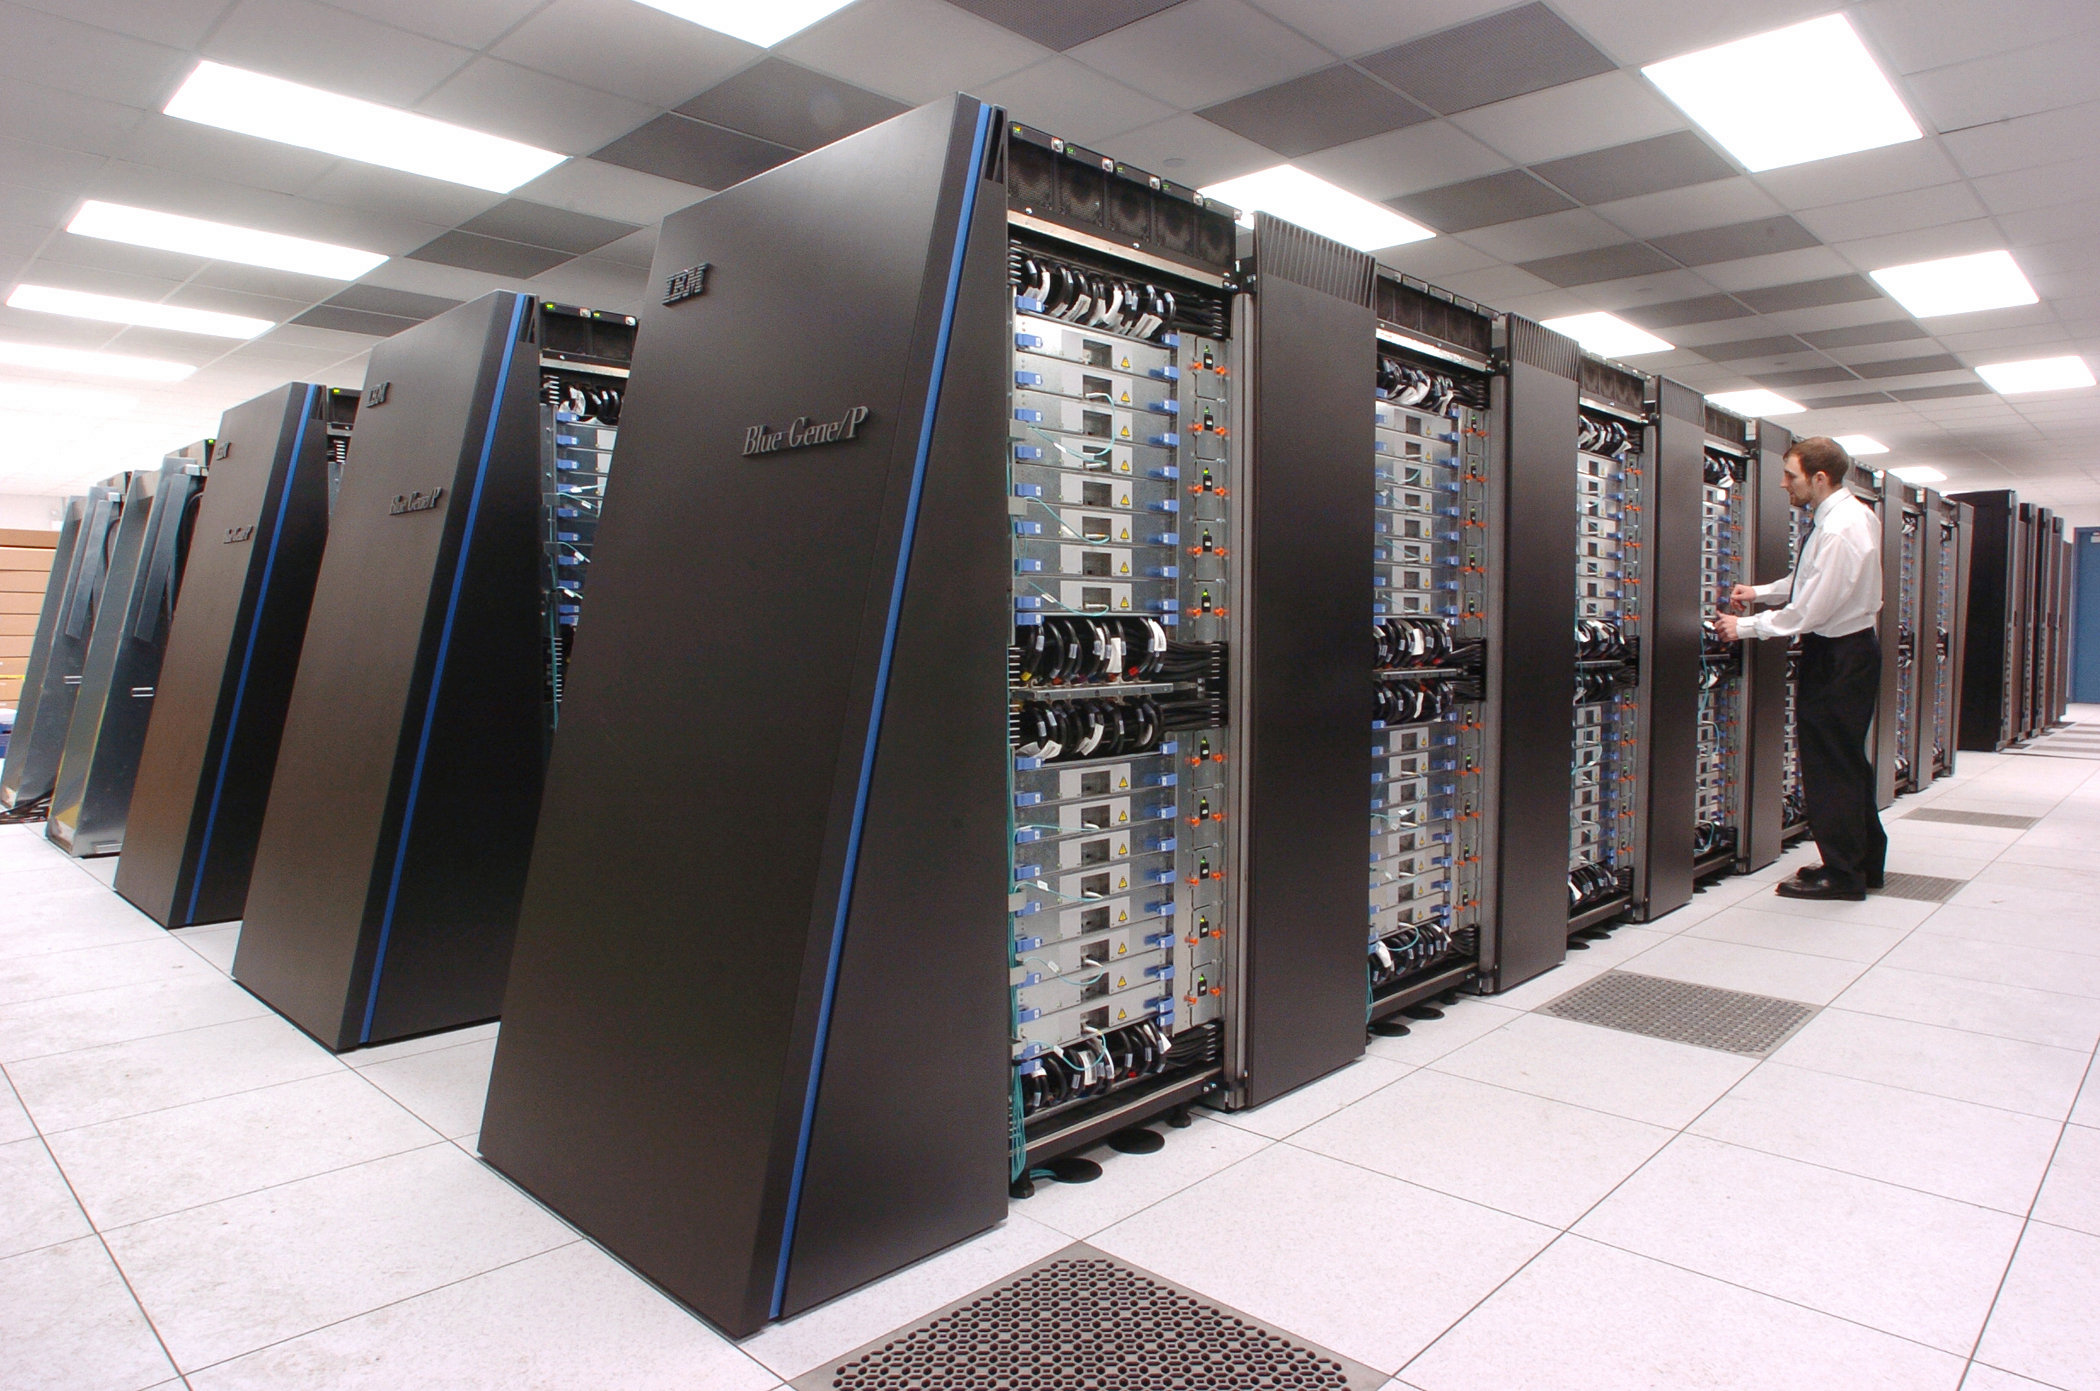
\includegraphics[width=\paperwidth]{imgs/ibm-blue-gene.jpg}}
\frame{}
}

{
\usebackgroundtemplate{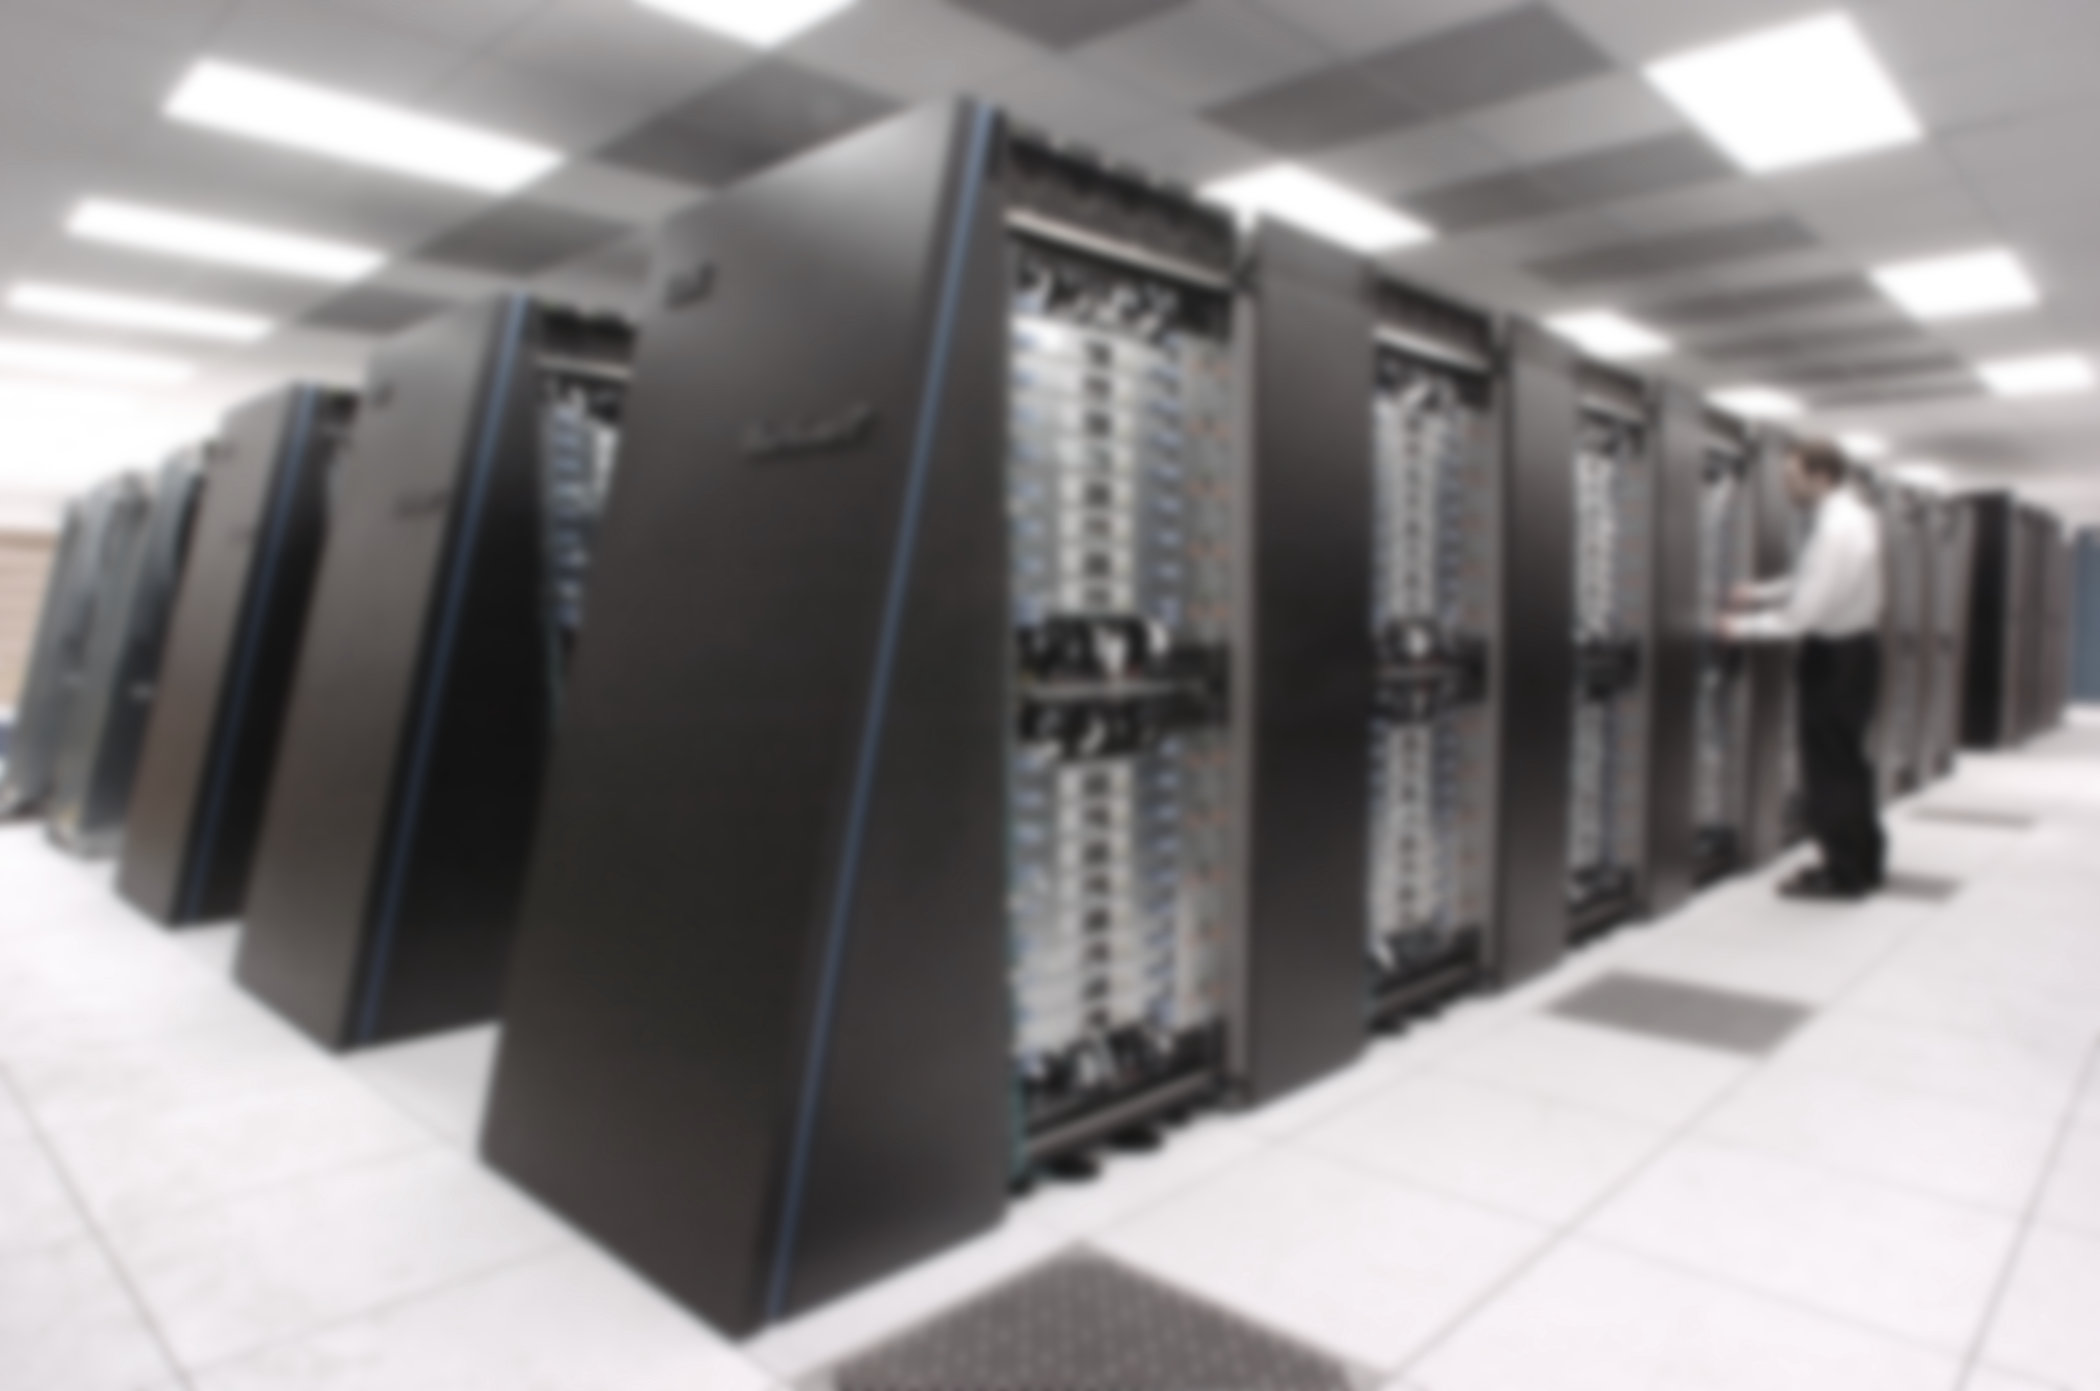
\includegraphics[width=\paperwidth]{imgs/ibm-blue-gene-back.jpg}}
\begin{frame}
\begin{block}{Computational Resources}
	\begin{itemize}
		\item super computer\pause
		\item computer cluster\pause
		\item computational grid\pause
		\item scientific cloud
	\end{itemize}
\end{block}
\end{frame}

\begin{frame}
\begin{block}{Grid Entities}
	\begin{itemize}
		\item virtual organisations
		\item resource providers
		\item grid maintainer/operator
	\end{itemize}
\end{block}
\end{frame}
}

\subsection{Marketplace}

{
\usebackgroundtemplate{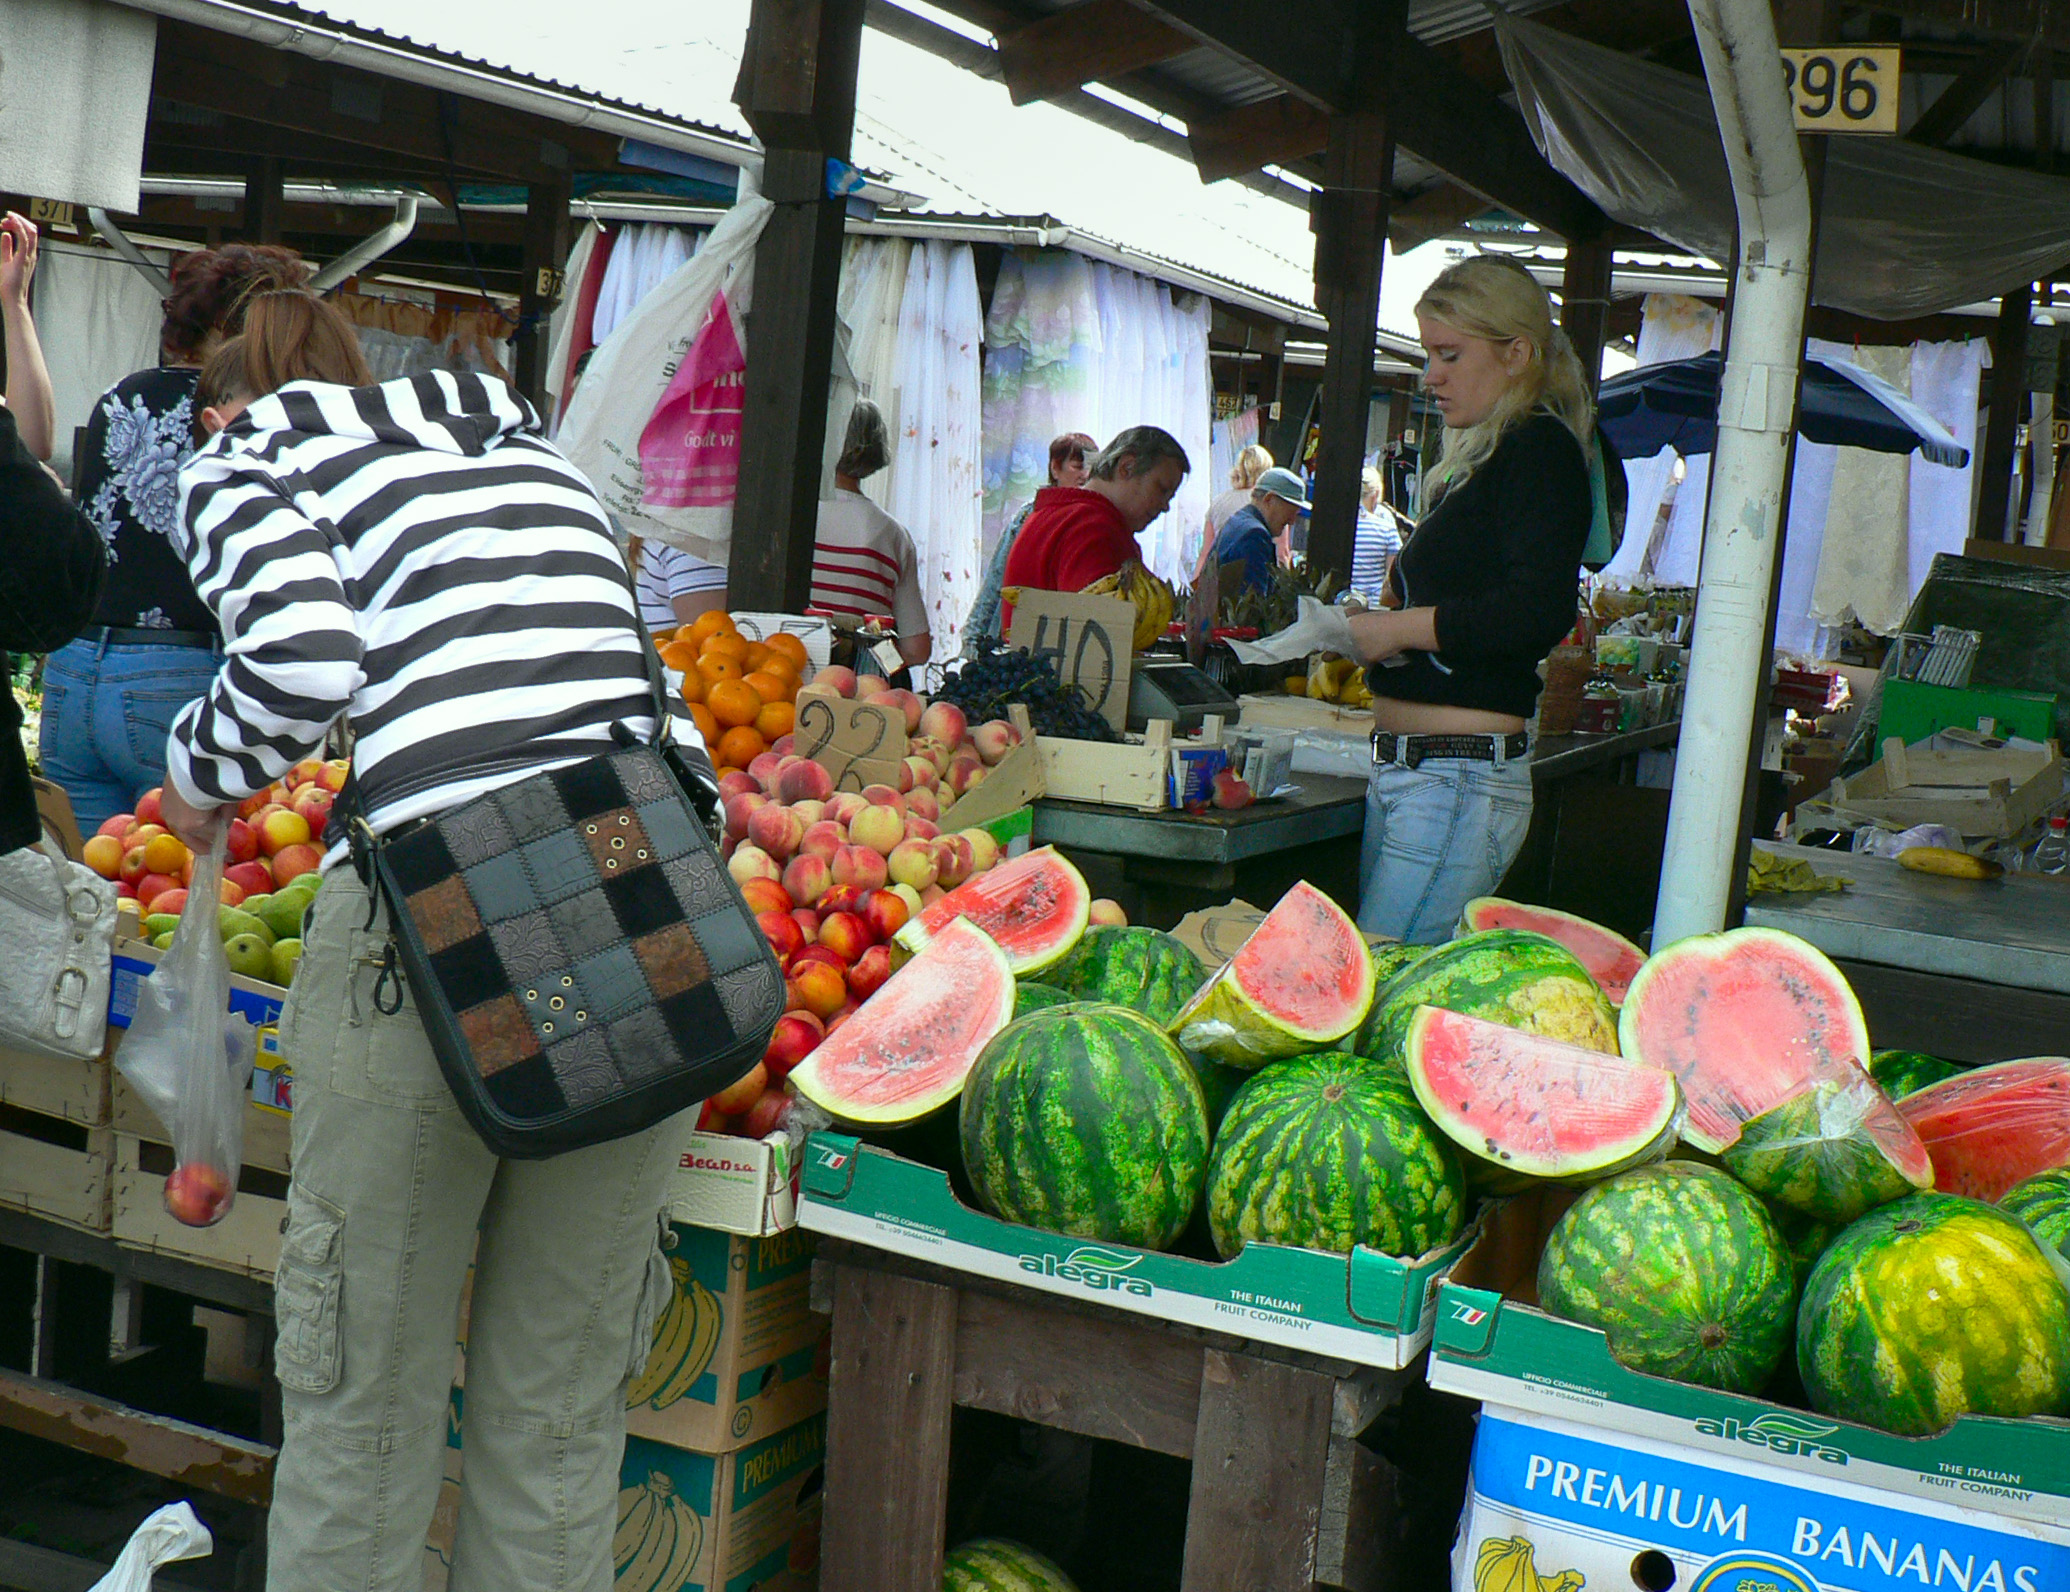
\includegraphics[width=\paperwidth]{imgs/marketplace.jpg}}
\frame{}
}

{
\usebackgroundtemplate{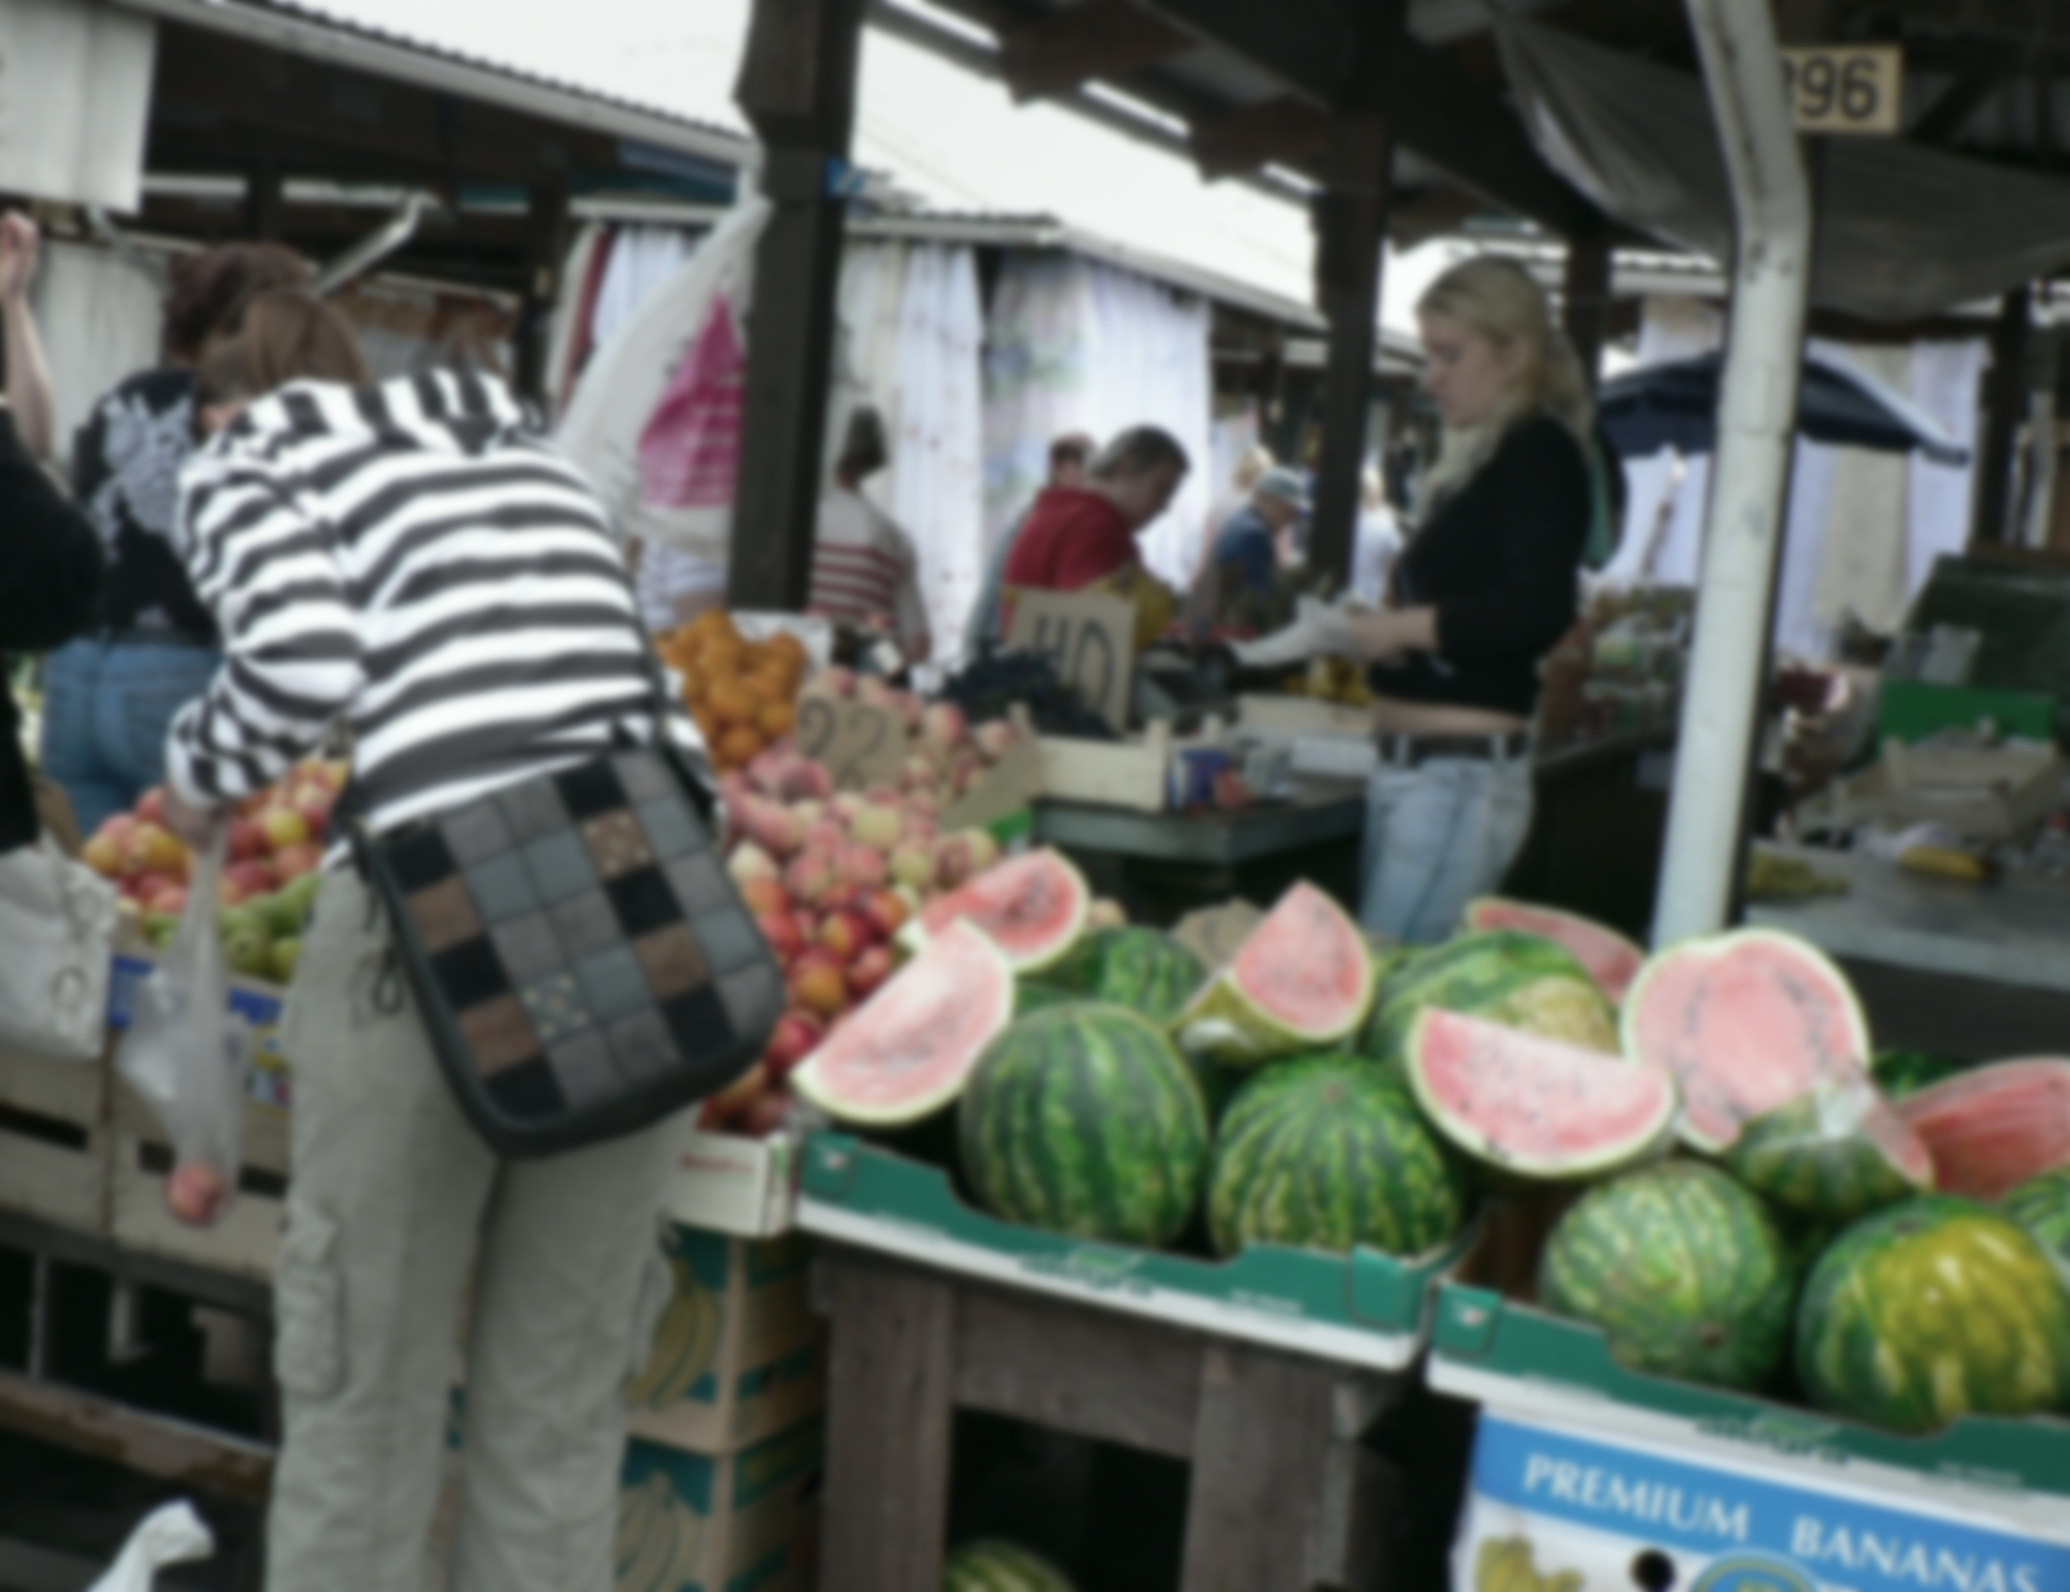
\includegraphics[width=\paperwidth]{imgs/marketplace-back.jpg}}
\begin{frame}
\begin{block}{Marketplace vs. GRID}
	\begin{description}
		\item[plain marketplace]{users with shell access, no control}\pause
		\item[central authority]{static allocation of resources, single point of access}
	\end{description}
\end{block}
\end{frame}
}

\section{Job Scheduling}
\subsection{The model}

\begin{frame}
	\frametitle{Job Scheduling}
	\center
	\begin{minipage}[b]{\textwidth}
		% Graphic for TeX using PGF
% Title: /home/simon/repos/teaching/talks/ia068_phd/schedule1.dia
% Creator: Dia v0.97.1
% CreationDate: Thu May 17 08:13:21 2012
% For: simon
% \usepackage{tikz}
% The following commands are not supported in PSTricks at present
% We define them conditionally, so when they are implemented,
% this pgf file will use them.
\ifx\du\undefined
  \newlength{\du}
\fi
\setlength{\du}{15\unitlength}
\begin{tikzpicture}
\pgftransformxscale{1.000000}
\pgftransformyscale{-1.000000}
\definecolor{dialinecolor}{rgb}{0.000000, 0.000000, 0.000000}
\pgfsetstrokecolor{dialinecolor}
\definecolor{dialinecolor}{rgb}{1.000000, 1.000000, 1.000000}
\pgfsetfillcolor{dialinecolor}
\definecolor{dialinecolor}{rgb}{1.000000, 1.000000, 1.000000}
\pgfsetfillcolor{dialinecolor}
\fill (5.000000\du,3.000000\du)--(5.000000\du,5.000000\du)--(11.000000\du,5.000000\du)--(11.000000\du,3.000000\du)--cycle;
\pgfsetlinewidth{0.100000\du}
\pgfsetdash{}{0pt}
\pgfsetdash{}{0pt}
\pgfsetmiterjoin
\definecolor{dialinecolor}{rgb}{0.000000, 0.000000, 0.000000}
\pgfsetstrokecolor{dialinecolor}
\draw (5.000000\du,3.000000\du)--(5.000000\du,5.000000\du)--(11.000000\du,5.000000\du)--(11.000000\du,3.000000\du)--cycle;
% setfont left to latex
\definecolor{dialinecolor}{rgb}{0.000000, 0.000000, 0.000000}
\pgfsetstrokecolor{dialinecolor}
\node at (8.000000\du,4.180000\du){Job1 length=3};
\definecolor{dialinecolor}{rgb}{1.000000, 1.000000, 1.000000}
\pgfsetfillcolor{dialinecolor}
\fill (12.000000\du,3.000000\du)--(12.000000\du,5.000000\du)--(18.000000\du,5.000000\du)--(18.000000\du,3.000000\du)--cycle;
\pgfsetlinewidth{0.100000\du}
\pgfsetdash{}{0pt}
\pgfsetdash{}{0pt}
\pgfsetmiterjoin
\definecolor{dialinecolor}{rgb}{0.000000, 0.000000, 0.000000}
\pgfsetstrokecolor{dialinecolor}
\draw (12.000000\du,3.000000\du)--(12.000000\du,5.000000\du)--(18.000000\du,5.000000\du)--(18.000000\du,3.000000\du)--cycle;
% setfont left to latex
\definecolor{dialinecolor}{rgb}{0.000000, 0.000000, 0.000000}
\pgfsetstrokecolor{dialinecolor}
\node at (15.000000\du,4.180000\du){Job2 length=3};
\definecolor{dialinecolor}{rgb}{1.000000, 1.000000, 1.000000}
\pgfsetfillcolor{dialinecolor}
\fill (5.000000\du,6.000000\du)--(5.000000\du,8.000000\du)--(17.000000\du,8.000000\du)--(17.000000\du,6.000000\du)--cycle;
\pgfsetlinewidth{0.100000\du}
\pgfsetdash{}{0pt}
\pgfsetdash{}{0pt}
\pgfsetmiterjoin
\definecolor{dialinecolor}{rgb}{0.000000, 0.000000, 0.000000}
\pgfsetstrokecolor{dialinecolor}
\draw (5.000000\du,6.000000\du)--(5.000000\du,8.000000\du)--(17.000000\du,8.000000\du)--(17.000000\du,6.000000\du)--cycle;
% setfont left to latex
\definecolor{dialinecolor}{rgb}{0.000000, 0.000000, 0.000000}
\pgfsetstrokecolor{dialinecolor}
\node at (11.000000\du,7.180000\du){Job3 length=6};
\definecolor{dialinecolor}{rgb}{1.000000, 1.000000, 1.000000}
\pgfsetfillcolor{dialinecolor}
\fill (18.000000\du,6.000000\du)--(18.000000\du,8.000000\du)--(30.000000\du,8.000000\du)--(30.000000\du,6.000000\du)--cycle;
\pgfsetlinewidth{0.100000\du}
\pgfsetdash{}{0pt}
\pgfsetdash{}{0pt}
\pgfsetmiterjoin
\definecolor{dialinecolor}{rgb}{0.000000, 0.000000, 0.000000}
\pgfsetstrokecolor{dialinecolor}
\draw (18.000000\du,6.000000\du)--(18.000000\du,8.000000\du)--(30.000000\du,8.000000\du)--(30.000000\du,6.000000\du)--cycle;
% setfont left to latex
\definecolor{dialinecolor}{rgb}{0.000000, 0.000000, 0.000000}
\pgfsetstrokecolor{dialinecolor}
\node at (24.000000\du,7.180000\du){Job4 length=6};
\definecolor{dialinecolor}{rgb}{1.000000, 1.000000, 1.000000}
\pgfsetfillcolor{dialinecolor}
\fill (5.000000\du,9.000000\du)--(5.000000\du,11.000000\du)--(23.000000\du,11.000000\du)--(23.000000\du,9.000000\du)--cycle;
\pgfsetlinewidth{0.100000\du}
\pgfsetdash{}{0pt}
\pgfsetdash{}{0pt}
\pgfsetmiterjoin
\definecolor{dialinecolor}{rgb}{0.000000, 0.000000, 0.000000}
\pgfsetstrokecolor{dialinecolor}
\draw (5.000000\du,9.000000\du)--(5.000000\du,11.000000\du)--(23.000000\du,11.000000\du)--(23.000000\du,9.000000\du)--cycle;
% setfont left to latex
\definecolor{dialinecolor}{rgb}{0.000000, 0.000000, 0.000000}
\pgfsetstrokecolor{dialinecolor}
\node at (14.000000\du,10.180000\du){Job5 length=9};
\end{tikzpicture}

	\end{minipage}
\end{frame}

\begin{frame}
	\frametitle{Job Scheduling}
	\center
	\begin{minipage}[b]{\textwidth}
		% Graphic for TeX using PGF
% Title: /home/simon/repos/teaching/talks/ia068_phd/schedule2.dia
% Creator: Dia v0.97.1
% CreationDate: Thu May 17 08:13:05 2012
% For: simon
% \usepackage{tikz}
% The following commands are not supported in PSTricks at present
% We define them conditionally, so when they are implemented,
% this pgf file will use them.
\ifx\du\undefined
  \newlength{\du}
\fi
\setlength{\du}{15\unitlength}
\begin{tikzpicture}
\pgftransformxscale{1.000000}
\pgftransformyscale{-1.000000}
\definecolor{dialinecolor}{rgb}{0.000000, 0.000000, 0.000000}
\pgfsetstrokecolor{dialinecolor}
\definecolor{dialinecolor}{rgb}{1.000000, 1.000000, 1.000000}
\pgfsetfillcolor{dialinecolor}
\definecolor{dialinecolor}{rgb}{1.000000, 1.000000, 1.000000}
\pgfsetfillcolor{dialinecolor}
\fill (17.000000\du,6.000000\du)--(17.000000\du,8.000000\du)--(23.000000\du,8.000000\du)--(23.000000\du,6.000000\du)--cycle;
\pgfsetlinewidth{0.100000\du}
\pgfsetdash{}{0pt}
\pgfsetdash{}{0pt}
\pgfsetmiterjoin
\definecolor{dialinecolor}{rgb}{0.000000, 0.000000, 0.000000}
\pgfsetstrokecolor{dialinecolor}
\draw (17.000000\du,6.000000\du)--(17.000000\du,8.000000\du)--(23.000000\du,8.000000\du)--(23.000000\du,6.000000\du)--cycle;
% setfont left to latex
\definecolor{dialinecolor}{rgb}{0.000000, 0.000000, 0.000000}
\pgfsetstrokecolor{dialinecolor}
\node at (20.000000\du,7.180000\du){Job1 length=3};
\definecolor{dialinecolor}{rgb}{1.000000, 1.000000, 1.000000}
\pgfsetfillcolor{dialinecolor}
\fill (17.000000\du,3.000000\du)--(17.000000\du,5.000000\du)--(23.000000\du,5.000000\du)--(23.000000\du,3.000000\du)--cycle;
\pgfsetlinewidth{0.100000\du}
\pgfsetdash{}{0pt}
\pgfsetdash{}{0pt}
\pgfsetmiterjoin
\definecolor{dialinecolor}{rgb}{0.000000, 0.000000, 0.000000}
\pgfsetstrokecolor{dialinecolor}
\draw (17.000000\du,3.000000\du)--(17.000000\du,5.000000\du)--(23.000000\du,5.000000\du)--(23.000000\du,3.000000\du)--cycle;
% setfont left to latex
\definecolor{dialinecolor}{rgb}{0.000000, 0.000000, 0.000000}
\pgfsetstrokecolor{dialinecolor}
\node at (20.000000\du,4.180000\du){Job2 length=3};
\definecolor{dialinecolor}{rgb}{1.000000, 1.000000, 1.000000}
\pgfsetfillcolor{dialinecolor}
\fill (5.000000\du,6.000000\du)--(5.000000\du,8.000000\du)--(17.000000\du,8.000000\du)--(17.000000\du,6.000000\du)--cycle;
\pgfsetlinewidth{0.100000\du}
\pgfsetdash{}{0pt}
\pgfsetdash{}{0pt}
\pgfsetmiterjoin
\definecolor{dialinecolor}{rgb}{0.000000, 0.000000, 0.000000}
\pgfsetstrokecolor{dialinecolor}
\draw (5.000000\du,6.000000\du)--(5.000000\du,8.000000\du)--(17.000000\du,8.000000\du)--(17.000000\du,6.000000\du)--cycle;
% setfont left to latex
\definecolor{dialinecolor}{rgb}{0.000000, 0.000000, 0.000000}
\pgfsetstrokecolor{dialinecolor}
\node at (11.000000\du,7.180000\du){Job3 length=6};
\definecolor{dialinecolor}{rgb}{1.000000, 1.000000, 1.000000}
\pgfsetfillcolor{dialinecolor}
\fill (5.000000\du,3.000000\du)--(5.000000\du,5.000000\du)--(17.000000\du,5.000000\du)--(17.000000\du,3.000000\du)--cycle;
\pgfsetlinewidth{0.100000\du}
\pgfsetdash{}{0pt}
\pgfsetdash{}{0pt}
\pgfsetmiterjoin
\definecolor{dialinecolor}{rgb}{0.000000, 0.000000, 0.000000}
\pgfsetstrokecolor{dialinecolor}
\draw (5.000000\du,3.000000\du)--(5.000000\du,5.000000\du)--(17.000000\du,5.000000\du)--(17.000000\du,3.000000\du)--cycle;
% setfont left to latex
\definecolor{dialinecolor}{rgb}{0.000000, 0.000000, 0.000000}
\pgfsetstrokecolor{dialinecolor}
\node at (11.000000\du,4.180000\du){Job4 length=6};
\definecolor{dialinecolor}{rgb}{1.000000, 1.000000, 1.000000}
\pgfsetfillcolor{dialinecolor}
\fill (5.000000\du,9.000000\du)--(5.000000\du,11.000000\du)--(23.000000\du,11.000000\du)--(23.000000\du,9.000000\du)--cycle;
\pgfsetlinewidth{0.100000\du}
\pgfsetdash{}{0pt}
\pgfsetdash{}{0pt}
\pgfsetmiterjoin
\definecolor{dialinecolor}{rgb}{0.000000, 0.000000, 0.000000}
\pgfsetstrokecolor{dialinecolor}
\draw (5.000000\du,9.000000\du)--(5.000000\du,11.000000\du)--(23.000000\du,11.000000\du)--(23.000000\du,9.000000\du)--cycle;
% setfont left to latex
\definecolor{dialinecolor}{rgb}{0.000000, 0.000000, 0.000000}
\pgfsetstrokecolor{dialinecolor}
\node at (14.000000\du,10.180000\du){Job5 length=9};
\pgfsetlinewidth{0.100000\du}
\pgfsetdash{}{0pt}
\pgfsetdash{}{0pt}
\pgfsetbuttcap
\pgfsetmiterjoin
\pgfsetlinewidth{0.100000\du}
\pgfsetbuttcap
\pgfsetmiterjoin
\pgfsetdash{}{0pt}
\definecolor{dialinecolor}{rgb}{0.000000, 0.000000, 0.000000}
\pgfsetstrokecolor{dialinecolor}
\draw (1.000000\du,3.000000\du)--(1.000000\du,5.000000\du);
\pgfsetbuttcap
\pgfsetmiterjoin
\pgfsetdash{}{0pt}
\definecolor{dialinecolor}{rgb}{0.000000, 0.000000, 0.000000}
\pgfsetstrokecolor{dialinecolor}
\draw (1.000000\du,3.000000\du)--(4.236842\du,3.000000\du);
\pgfsetbuttcap
\pgfsetmiterjoin
\pgfsetdash{}{0pt}
\definecolor{dialinecolor}{rgb}{0.000000, 0.000000, 0.000000}
\pgfsetstrokecolor{dialinecolor}
\draw (1.000000\du,5.000000\du)--(4.236842\du,5.000000\du);
% setfont left to latex
\definecolor{dialinecolor}{rgb}{0.000000, 0.000000, 0.000000}
\pgfsetstrokecolor{dialinecolor}
\node at (2.699342\du,4.250000\du){machine1};
\pgfsetlinewidth{0.100000\du}
\pgfsetdash{}{0pt}
\pgfsetdash{}{0pt}
\pgfsetbuttcap
\pgfsetmiterjoin
\pgfsetlinewidth{0.100000\du}
\pgfsetbuttcap
\pgfsetmiterjoin
\pgfsetdash{}{0pt}
\definecolor{dialinecolor}{rgb}{0.000000, 0.000000, 0.000000}
\pgfsetstrokecolor{dialinecolor}
\draw (1.000000\du,6.000000\du)--(1.000000\du,8.000000\du);
\pgfsetbuttcap
\pgfsetmiterjoin
\pgfsetdash{}{0pt}
\definecolor{dialinecolor}{rgb}{0.000000, 0.000000, 0.000000}
\pgfsetstrokecolor{dialinecolor}
\draw (1.000000\du,6.000000\du)--(4.236842\du,6.000000\du);
\pgfsetbuttcap
\pgfsetmiterjoin
\pgfsetdash{}{0pt}
\definecolor{dialinecolor}{rgb}{0.000000, 0.000000, 0.000000}
\pgfsetstrokecolor{dialinecolor}
\draw (1.000000\du,8.000000\du)--(4.236842\du,8.000000\du);
% setfont left to latex
\definecolor{dialinecolor}{rgb}{0.000000, 0.000000, 0.000000}
\pgfsetstrokecolor{dialinecolor}
\node at (2.699342\du,7.250000\du){machine2};
\pgfsetlinewidth{0.100000\du}
\pgfsetdash{}{0pt}
\pgfsetdash{}{0pt}
\pgfsetbuttcap
\pgfsetmiterjoin
\pgfsetlinewidth{0.100000\du}
\pgfsetbuttcap
\pgfsetmiterjoin
\pgfsetdash{}{0pt}
\definecolor{dialinecolor}{rgb}{0.000000, 0.000000, 0.000000}
\pgfsetstrokecolor{dialinecolor}
\draw (1.000000\du,9.000000\du)--(1.000000\du,11.000000\du);
\pgfsetbuttcap
\pgfsetmiterjoin
\pgfsetdash{}{0pt}
\definecolor{dialinecolor}{rgb}{0.000000, 0.000000, 0.000000}
\pgfsetstrokecolor{dialinecolor}
\draw (1.000000\du,9.000000\du)--(4.236842\du,9.000000\du);
\pgfsetbuttcap
\pgfsetmiterjoin
\pgfsetdash{}{0pt}
\definecolor{dialinecolor}{rgb}{0.000000, 0.000000, 0.000000}
\pgfsetstrokecolor{dialinecolor}
\draw (1.000000\du,11.000000\du)--(4.236842\du,11.000000\du);
% setfont left to latex
\definecolor{dialinecolor}{rgb}{0.000000, 0.000000, 0.000000}
\pgfsetstrokecolor{dialinecolor}
\node at (2.699342\du,10.250000\du){machine3};
\end{tikzpicture}

	\end{minipage}
\end{frame}

\subsection{Issues}

\begin{frame}
	\frametitle{Multi-dimensionality}
	\begin{itemize}
		\item jobs require specific properties from nodes
		\item jobs have more dimensions than length
		\begin{itemize}
			\item number of cpus
			\item amount of memory
			\item number of gpus
		\end{itemize}
		\item virtualized nodes can be started in different configurations
	\end{itemize}
\end{frame}

\begin{frame}
	\frametitle{Non-clairvoyance}
	\begin{itemize}
		\item specified job length is the upper limit
		\begin{itemize}
			\item 24 hour job can still run 5 minutes
		\end{itemize}
	\end{itemize}
\end{frame}

\begin{frame}
	\frametitle{Non-clairvoyance}
	\center
	\begin{minipage}[b]{\textwidth}
		% Graphic for TeX using PGF
% Title: /home/simon/repos/teaching/talks/ia068_phd/schedule3.dia
% Creator: Dia v0.97.1
% CreationDate: Thu May 17 08:25:27 2012
% For: simon
% \usepackage{tikz}
% The following commands are not supported in PSTricks at present
% We define them conditionally, so when they are implemented,
% this pgf file will use them.
\ifx\du\undefined
  \newlength{\du}
\fi
\setlength{\du}{15\unitlength}
\begin{tikzpicture}
\pgftransformxscale{1.000000}
\pgftransformyscale{-1.000000}
\definecolor{dialinecolor}{rgb}{0.000000, 0.000000, 0.000000}
\pgfsetstrokecolor{dialinecolor}
\definecolor{dialinecolor}{rgb}{1.000000, 1.000000, 1.000000}
\pgfsetfillcolor{dialinecolor}
\definecolor{dialinecolor}{rgb}{1.000000, 1.000000, 1.000000}
\pgfsetfillcolor{dialinecolor}
\fill (10.000000\du,6.000000\du)--(10.000000\du,8.000000\du)--(14.000000\du,8.000000\du)--(14.000000\du,6.000000\du)--cycle;
\pgfsetlinewidth{0.100000\du}
\pgfsetdash{}{0pt}
\pgfsetdash{}{0pt}
\pgfsetmiterjoin
\definecolor{dialinecolor}{rgb}{0.000000, 0.000000, 0.000000}
\pgfsetstrokecolor{dialinecolor}
\draw (10.000000\du,6.000000\du)--(10.000000\du,8.000000\du)--(14.000000\du,8.000000\du)--(14.000000\du,6.000000\du)--cycle;
% setfont left to latex
\definecolor{dialinecolor}{rgb}{0.000000, 0.000000, 0.000000}
\pgfsetstrokecolor{dialinecolor}
\node at (12.000000\du,7.180000\du){Job1};
\definecolor{dialinecolor}{rgb}{1.000000, 1.000000, 1.000000}
\pgfsetfillcolor{dialinecolor}
\fill (11.000000\du,3.000000\du)--(11.000000\du,5.000000\du)--(14.000000\du,5.000000\du)--(14.000000\du,3.000000\du)--cycle;
\pgfsetlinewidth{0.100000\du}
\pgfsetdash{}{0pt}
\pgfsetdash{}{0pt}
\pgfsetmiterjoin
\definecolor{dialinecolor}{rgb}{0.000000, 0.000000, 0.000000}
\pgfsetstrokecolor{dialinecolor}
\draw (11.000000\du,3.000000\du)--(11.000000\du,5.000000\du)--(14.000000\du,5.000000\du)--(14.000000\du,3.000000\du)--cycle;
% setfont left to latex
\definecolor{dialinecolor}{rgb}{0.000000, 0.000000, 0.000000}
\pgfsetstrokecolor{dialinecolor}
\node at (12.500000\du,4.180000\du){Job2};
\definecolor{dialinecolor}{rgb}{1.000000, 1.000000, 1.000000}
\pgfsetfillcolor{dialinecolor}
\fill (5.000000\du,6.000000\du)--(5.000000\du,8.000000\du)--(10.000000\du,8.000000\du)--(10.000000\du,6.000000\du)--cycle;
\pgfsetlinewidth{0.100000\du}
\pgfsetdash{}{0pt}
\pgfsetdash{}{0pt}
\pgfsetmiterjoin
\definecolor{dialinecolor}{rgb}{0.000000, 0.000000, 0.000000}
\pgfsetstrokecolor{dialinecolor}
\draw (5.000000\du,6.000000\du)--(5.000000\du,8.000000\du)--(10.000000\du,8.000000\du)--(10.000000\du,6.000000\du)--cycle;
% setfont left to latex
\definecolor{dialinecolor}{rgb}{0.000000, 0.000000, 0.000000}
\pgfsetstrokecolor{dialinecolor}
\node at (7.500000\du,7.180000\du){Job3};
\definecolor{dialinecolor}{rgb}{1.000000, 1.000000, 1.000000}
\pgfsetfillcolor{dialinecolor}
\fill (5.000000\du,3.000000\du)--(5.000000\du,5.000000\du)--(11.000000\du,5.000000\du)--(11.000000\du,3.000000\du)--cycle;
\pgfsetlinewidth{0.100000\du}
\pgfsetdash{}{0pt}
\pgfsetdash{}{0pt}
\pgfsetmiterjoin
\definecolor{dialinecolor}{rgb}{0.000000, 0.000000, 0.000000}
\pgfsetstrokecolor{dialinecolor}
\draw (5.000000\du,3.000000\du)--(5.000000\du,5.000000\du)--(11.000000\du,5.000000\du)--(11.000000\du,3.000000\du)--cycle;
% setfont left to latex
\definecolor{dialinecolor}{rgb}{0.000000, 0.000000, 0.000000}
\pgfsetstrokecolor{dialinecolor}
\node at (8.000000\du,4.180000\du){Job4};
\definecolor{dialinecolor}{rgb}{1.000000, 1.000000, 1.000000}
\pgfsetfillcolor{dialinecolor}
\fill (5.000000\du,9.000000\du)--(5.000000\du,11.000000\du)--(23.000000\du,11.000000\du)--(23.000000\du,9.000000\du)--cycle;
\pgfsetlinewidth{0.100000\du}
\pgfsetdash{}{0pt}
\pgfsetdash{}{0pt}
\pgfsetmiterjoin
\definecolor{dialinecolor}{rgb}{0.000000, 0.000000, 0.000000}
\pgfsetstrokecolor{dialinecolor}
\draw (5.000000\du,9.000000\du)--(5.000000\du,11.000000\du)--(23.000000\du,11.000000\du)--(23.000000\du,9.000000\du)--cycle;
% setfont left to latex
\definecolor{dialinecolor}{rgb}{0.000000, 0.000000, 0.000000}
\pgfsetstrokecolor{dialinecolor}
\node at (14.000000\du,10.180000\du){Job5};
\pgfsetlinewidth{0.100000\du}
\pgfsetdash{}{0pt}
\pgfsetdash{}{0pt}
\pgfsetbuttcap
\pgfsetmiterjoin
\pgfsetlinewidth{0.100000\du}
\pgfsetbuttcap
\pgfsetmiterjoin
\pgfsetdash{}{0pt}
\definecolor{dialinecolor}{rgb}{0.000000, 0.000000, 0.000000}
\pgfsetstrokecolor{dialinecolor}
\draw (1.000000\du,3.000000\du)--(1.000000\du,5.000000\du);
\pgfsetbuttcap
\pgfsetmiterjoin
\pgfsetdash{}{0pt}
\definecolor{dialinecolor}{rgb}{0.000000, 0.000000, 0.000000}
\pgfsetstrokecolor{dialinecolor}
\draw (1.000000\du,3.000000\du)--(4.236842\du,3.000000\du);
\pgfsetbuttcap
\pgfsetmiterjoin
\pgfsetdash{}{0pt}
\definecolor{dialinecolor}{rgb}{0.000000, 0.000000, 0.000000}
\pgfsetstrokecolor{dialinecolor}
\draw (1.000000\du,5.000000\du)--(4.236842\du,5.000000\du);
% setfont left to latex
\definecolor{dialinecolor}{rgb}{0.000000, 0.000000, 0.000000}
\pgfsetstrokecolor{dialinecolor}
\node at (2.699342\du,4.210000\du){machine1};
\pgfsetlinewidth{0.100000\du}
\pgfsetdash{}{0pt}
\pgfsetdash{}{0pt}
\pgfsetbuttcap
\pgfsetmiterjoin
\pgfsetlinewidth{0.100000\du}
\pgfsetbuttcap
\pgfsetmiterjoin
\pgfsetdash{}{0pt}
\definecolor{dialinecolor}{rgb}{0.000000, 0.000000, 0.000000}
\pgfsetstrokecolor{dialinecolor}
\draw (1.000000\du,6.000000\du)--(1.000000\du,8.000000\du);
\pgfsetbuttcap
\pgfsetmiterjoin
\pgfsetdash{}{0pt}
\definecolor{dialinecolor}{rgb}{0.000000, 0.000000, 0.000000}
\pgfsetstrokecolor{dialinecolor}
\draw (1.000000\du,6.000000\du)--(4.236842\du,6.000000\du);
\pgfsetbuttcap
\pgfsetmiterjoin
\pgfsetdash{}{0pt}
\definecolor{dialinecolor}{rgb}{0.000000, 0.000000, 0.000000}
\pgfsetstrokecolor{dialinecolor}
\draw (1.000000\du,8.000000\du)--(4.236842\du,8.000000\du);
% setfont left to latex
\definecolor{dialinecolor}{rgb}{0.000000, 0.000000, 0.000000}
\pgfsetstrokecolor{dialinecolor}
\node at (2.699342\du,7.210000\du){machine2};
\pgfsetlinewidth{0.100000\du}
\pgfsetdash{}{0pt}
\pgfsetdash{}{0pt}
\pgfsetbuttcap
\pgfsetmiterjoin
\pgfsetlinewidth{0.100000\du}
\pgfsetbuttcap
\pgfsetmiterjoin
\pgfsetdash{}{0pt}
\definecolor{dialinecolor}{rgb}{0.000000, 0.000000, 0.000000}
\pgfsetstrokecolor{dialinecolor}
\draw (1.000000\du,9.000000\du)--(1.000000\du,11.000000\du);
\pgfsetbuttcap
\pgfsetmiterjoin
\pgfsetdash{}{0pt}
\definecolor{dialinecolor}{rgb}{0.000000, 0.000000, 0.000000}
\pgfsetstrokecolor{dialinecolor}
\draw (1.000000\du,9.000000\du)--(4.236842\du,9.000000\du);
\pgfsetbuttcap
\pgfsetmiterjoin
\pgfsetdash{}{0pt}
\definecolor{dialinecolor}{rgb}{0.000000, 0.000000, 0.000000}
\pgfsetstrokecolor{dialinecolor}
\draw (1.000000\du,11.000000\du)--(4.236842\du,11.000000\du);
% setfont left to latex
\definecolor{dialinecolor}{rgb}{0.000000, 0.000000, 0.000000}
\pgfsetstrokecolor{dialinecolor}
\node at (2.699342\du,10.210000\du){machine3};
\end{tikzpicture}

	\end{minipage}
\end{frame}

\begin{frame}
	\frametitle{Non-clairvoyance}
	\center
	\begin{minipage}[b]{\textwidth}
		% Graphic for TeX using PGF
% Title: /home/simon/repos/teaching/talks/ia068_phd/schedule4.dia
% Creator: Dia v0.97.1
% CreationDate: Thu May 17 08:25:43 2012
% For: simon
% \usepackage{tikz}
% The following commands are not supported in PSTricks at present
% We define them conditionally, so when they are implemented,
% this pgf file will use them.
\ifx\du\undefined
  \newlength{\du}
\fi
\setlength{\du}{15\unitlength}
\begin{tikzpicture}
\pgftransformxscale{1.000000}
\pgftransformyscale{-1.000000}
\definecolor{dialinecolor}{rgb}{0.000000, 0.000000, 0.000000}
\pgfsetstrokecolor{dialinecolor}
\definecolor{dialinecolor}{rgb}{1.000000, 1.000000, 1.000000}
\pgfsetfillcolor{dialinecolor}
\definecolor{dialinecolor}{rgb}{1.000000, 1.000000, 1.000000}
\pgfsetfillcolor{dialinecolor}
\fill (10.000000\du,6.000000\du)--(10.000000\du,8.000000\du)--(14.000000\du,8.000000\du)--(14.000000\du,6.000000\du)--cycle;
\pgfsetlinewidth{0.100000\du}
\pgfsetdash{}{0pt}
\pgfsetdash{}{0pt}
\pgfsetmiterjoin
\definecolor{dialinecolor}{rgb}{0.000000, 0.000000, 0.000000}
\pgfsetstrokecolor{dialinecolor}
\draw (10.000000\du,6.000000\du)--(10.000000\du,8.000000\du)--(14.000000\du,8.000000\du)--(14.000000\du,6.000000\du)--cycle;
% setfont left to latex
\definecolor{dialinecolor}{rgb}{0.000000, 0.000000, 0.000000}
\pgfsetstrokecolor{dialinecolor}
\node at (12.000000\du,7.180000\du){Job1};
\definecolor{dialinecolor}{rgb}{1.000000, 1.000000, 1.000000}
\pgfsetfillcolor{dialinecolor}
\fill (20.000000\du,6.000000\du)--(20.000000\du,8.000000\du)--(23.000000\du,8.000000\du)--(23.000000\du,6.000000\du)--cycle;
\pgfsetlinewidth{0.100000\du}
\pgfsetdash{}{0pt}
\pgfsetdash{}{0pt}
\pgfsetmiterjoin
\definecolor{dialinecolor}{rgb}{0.000000, 0.000000, 0.000000}
\pgfsetstrokecolor{dialinecolor}
\draw (20.000000\du,6.000000\du)--(20.000000\du,8.000000\du)--(23.000000\du,8.000000\du)--(23.000000\du,6.000000\du)--cycle;
% setfont left to latex
\definecolor{dialinecolor}{rgb}{0.000000, 0.000000, 0.000000}
\pgfsetstrokecolor{dialinecolor}
\node at (21.500000\du,7.180000\du){Job2};
\definecolor{dialinecolor}{rgb}{1.000000, 1.000000, 1.000000}
\pgfsetfillcolor{dialinecolor}
\fill (5.000000\du,6.000000\du)--(5.000000\du,8.000000\du)--(10.000000\du,8.000000\du)--(10.000000\du,6.000000\du)--cycle;
\pgfsetlinewidth{0.100000\du}
\pgfsetdash{}{0pt}
\pgfsetdash{}{0pt}
\pgfsetmiterjoin
\definecolor{dialinecolor}{rgb}{0.000000, 0.000000, 0.000000}
\pgfsetstrokecolor{dialinecolor}
\draw (5.000000\du,6.000000\du)--(5.000000\du,8.000000\du)--(10.000000\du,8.000000\du)--(10.000000\du,6.000000\du)--cycle;
% setfont left to latex
\definecolor{dialinecolor}{rgb}{0.000000, 0.000000, 0.000000}
\pgfsetstrokecolor{dialinecolor}
\node at (7.500000\du,7.180000\du){Job3};
\definecolor{dialinecolor}{rgb}{1.000000, 1.000000, 1.000000}
\pgfsetfillcolor{dialinecolor}
\fill (14.000000\du,6.000000\du)--(14.000000\du,8.000000\du)--(20.000000\du,8.000000\du)--(20.000000\du,6.000000\du)--cycle;
\pgfsetlinewidth{0.100000\du}
\pgfsetdash{}{0pt}
\pgfsetdash{}{0pt}
\pgfsetmiterjoin
\definecolor{dialinecolor}{rgb}{0.000000, 0.000000, 0.000000}
\pgfsetstrokecolor{dialinecolor}
\draw (14.000000\du,6.000000\du)--(14.000000\du,8.000000\du)--(20.000000\du,8.000000\du)--(20.000000\du,6.000000\du)--cycle;
% setfont left to latex
\definecolor{dialinecolor}{rgb}{0.000000, 0.000000, 0.000000}
\pgfsetstrokecolor{dialinecolor}
\node at (17.000000\du,7.180000\du){Job4};
\definecolor{dialinecolor}{rgb}{1.000000, 1.000000, 1.000000}
\pgfsetfillcolor{dialinecolor}
\fill (5.000000\du,9.000000\du)--(5.000000\du,11.000000\du)--(23.000000\du,11.000000\du)--(23.000000\du,9.000000\du)--cycle;
\pgfsetlinewidth{0.100000\du}
\pgfsetdash{}{0pt}
\pgfsetdash{}{0pt}
\pgfsetmiterjoin
\definecolor{dialinecolor}{rgb}{0.000000, 0.000000, 0.000000}
\pgfsetstrokecolor{dialinecolor}
\draw (5.000000\du,9.000000\du)--(5.000000\du,11.000000\du)--(23.000000\du,11.000000\du)--(23.000000\du,9.000000\du)--cycle;
% setfont left to latex
\definecolor{dialinecolor}{rgb}{0.000000, 0.000000, 0.000000}
\pgfsetstrokecolor{dialinecolor}
\node at (14.000000\du,10.180000\du){Job5};
\pgfsetlinewidth{0.100000\du}
\pgfsetdash{}{0pt}
\pgfsetdash{}{0pt}
\pgfsetbuttcap
\pgfsetmiterjoin
\pgfsetlinewidth{0.100000\du}
\pgfsetbuttcap
\pgfsetmiterjoin
\pgfsetdash{}{0pt}
\definecolor{dialinecolor}{rgb}{0.000000, 0.000000, 0.000000}
\pgfsetstrokecolor{dialinecolor}
\draw (1.000000\du,3.000000\du)--(1.000000\du,5.000000\du);
\pgfsetbuttcap
\pgfsetmiterjoin
\pgfsetdash{}{0pt}
\definecolor{dialinecolor}{rgb}{0.000000, 0.000000, 0.000000}
\pgfsetstrokecolor{dialinecolor}
\draw (1.000000\du,3.000000\du)--(4.236842\du,3.000000\du);
\pgfsetbuttcap
\pgfsetmiterjoin
\pgfsetdash{}{0pt}
\definecolor{dialinecolor}{rgb}{0.000000, 0.000000, 0.000000}
\pgfsetstrokecolor{dialinecolor}
\draw (1.000000\du,5.000000\du)--(4.236842\du,5.000000\du);
% setfont left to latex
\definecolor{dialinecolor}{rgb}{0.000000, 0.000000, 0.000000}
\pgfsetstrokecolor{dialinecolor}
\node at (2.699342\du,4.210000\du){machine1};
\pgfsetlinewidth{0.100000\du}
\pgfsetdash{}{0pt}
\pgfsetdash{}{0pt}
\pgfsetbuttcap
\pgfsetmiterjoin
\pgfsetlinewidth{0.100000\du}
\pgfsetbuttcap
\pgfsetmiterjoin
\pgfsetdash{}{0pt}
\definecolor{dialinecolor}{rgb}{0.000000, 0.000000, 0.000000}
\pgfsetstrokecolor{dialinecolor}
\draw (1.000000\du,6.000000\du)--(1.000000\du,8.000000\du);
\pgfsetbuttcap
\pgfsetmiterjoin
\pgfsetdash{}{0pt}
\definecolor{dialinecolor}{rgb}{0.000000, 0.000000, 0.000000}
\pgfsetstrokecolor{dialinecolor}
\draw (1.000000\du,6.000000\du)--(4.236842\du,6.000000\du);
\pgfsetbuttcap
\pgfsetmiterjoin
\pgfsetdash{}{0pt}
\definecolor{dialinecolor}{rgb}{0.000000, 0.000000, 0.000000}
\pgfsetstrokecolor{dialinecolor}
\draw (1.000000\du,8.000000\du)--(4.236842\du,8.000000\du);
% setfont left to latex
\definecolor{dialinecolor}{rgb}{0.000000, 0.000000, 0.000000}
\pgfsetstrokecolor{dialinecolor}
\node at (2.699342\du,7.210000\du){machine2};
\pgfsetlinewidth{0.100000\du}
\pgfsetdash{}{0pt}
\pgfsetdash{}{0pt}
\pgfsetbuttcap
\pgfsetmiterjoin
\pgfsetlinewidth{0.100000\du}
\pgfsetbuttcap
\pgfsetmiterjoin
\pgfsetdash{}{0pt}
\definecolor{dialinecolor}{rgb}{0.000000, 0.000000, 0.000000}
\pgfsetstrokecolor{dialinecolor}
\draw (1.000000\du,9.000000\du)--(1.000000\du,11.000000\du);
\pgfsetbuttcap
\pgfsetmiterjoin
\pgfsetdash{}{0pt}
\definecolor{dialinecolor}{rgb}{0.000000, 0.000000, 0.000000}
\pgfsetstrokecolor{dialinecolor}
\draw (1.000000\du,9.000000\du)--(4.236842\du,9.000000\du);
\pgfsetbuttcap
\pgfsetmiterjoin
\pgfsetdash{}{0pt}
\definecolor{dialinecolor}{rgb}{0.000000, 0.000000, 0.000000}
\pgfsetstrokecolor{dialinecolor}
\draw (1.000000\du,11.000000\du)--(4.236842\du,11.000000\du);
% setfont left to latex
\definecolor{dialinecolor}{rgb}{0.000000, 0.000000, 0.000000}
\pgfsetstrokecolor{dialinecolor}
\node at (2.699342\du,10.210000\du){machine3};
\end{tikzpicture}

	\end{minipage}
\end{frame}

\begin{frame}
	\frametitle{On-line scheduling}
	\begin{itemize}
		\item at any point of time a new job can arrive
		\item we can't saturate the grid
	\end{itemize}
\end{frame}

{
\usebackgroundtemplate{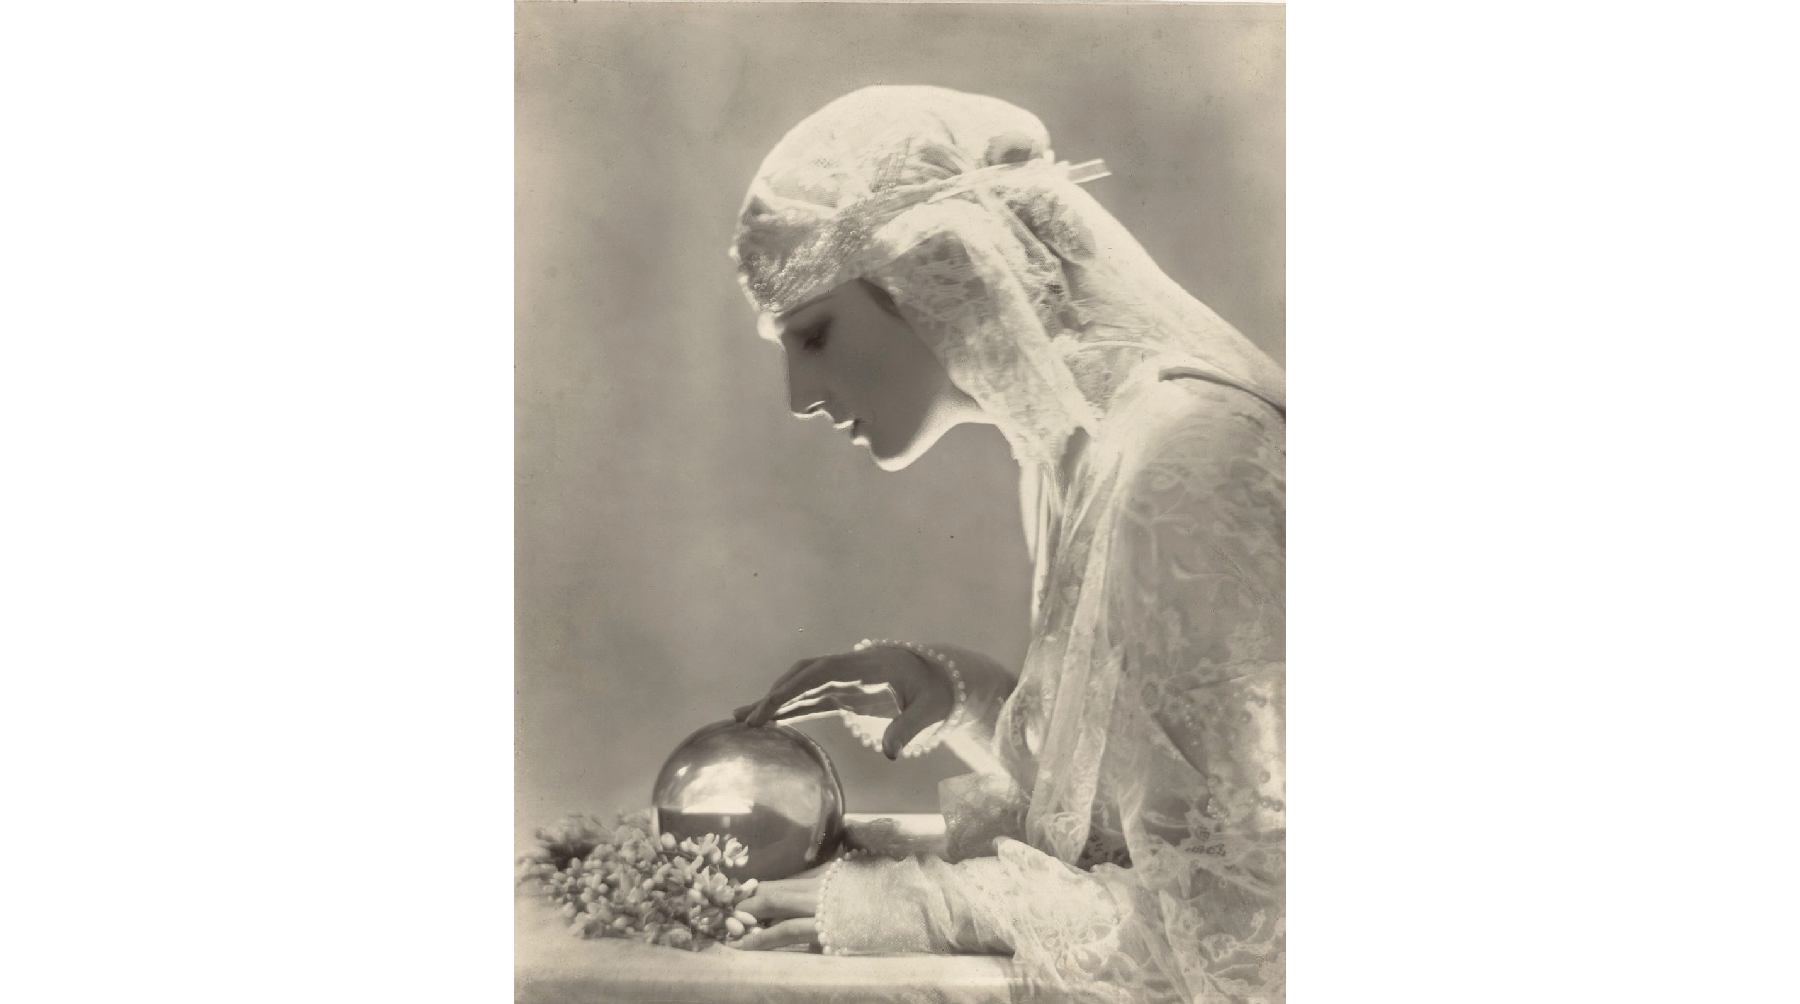
\includegraphics[width=\paperwidth]{imgs/oracle2.png}}
\frame{}
}

{
\usebackgroundtemplate{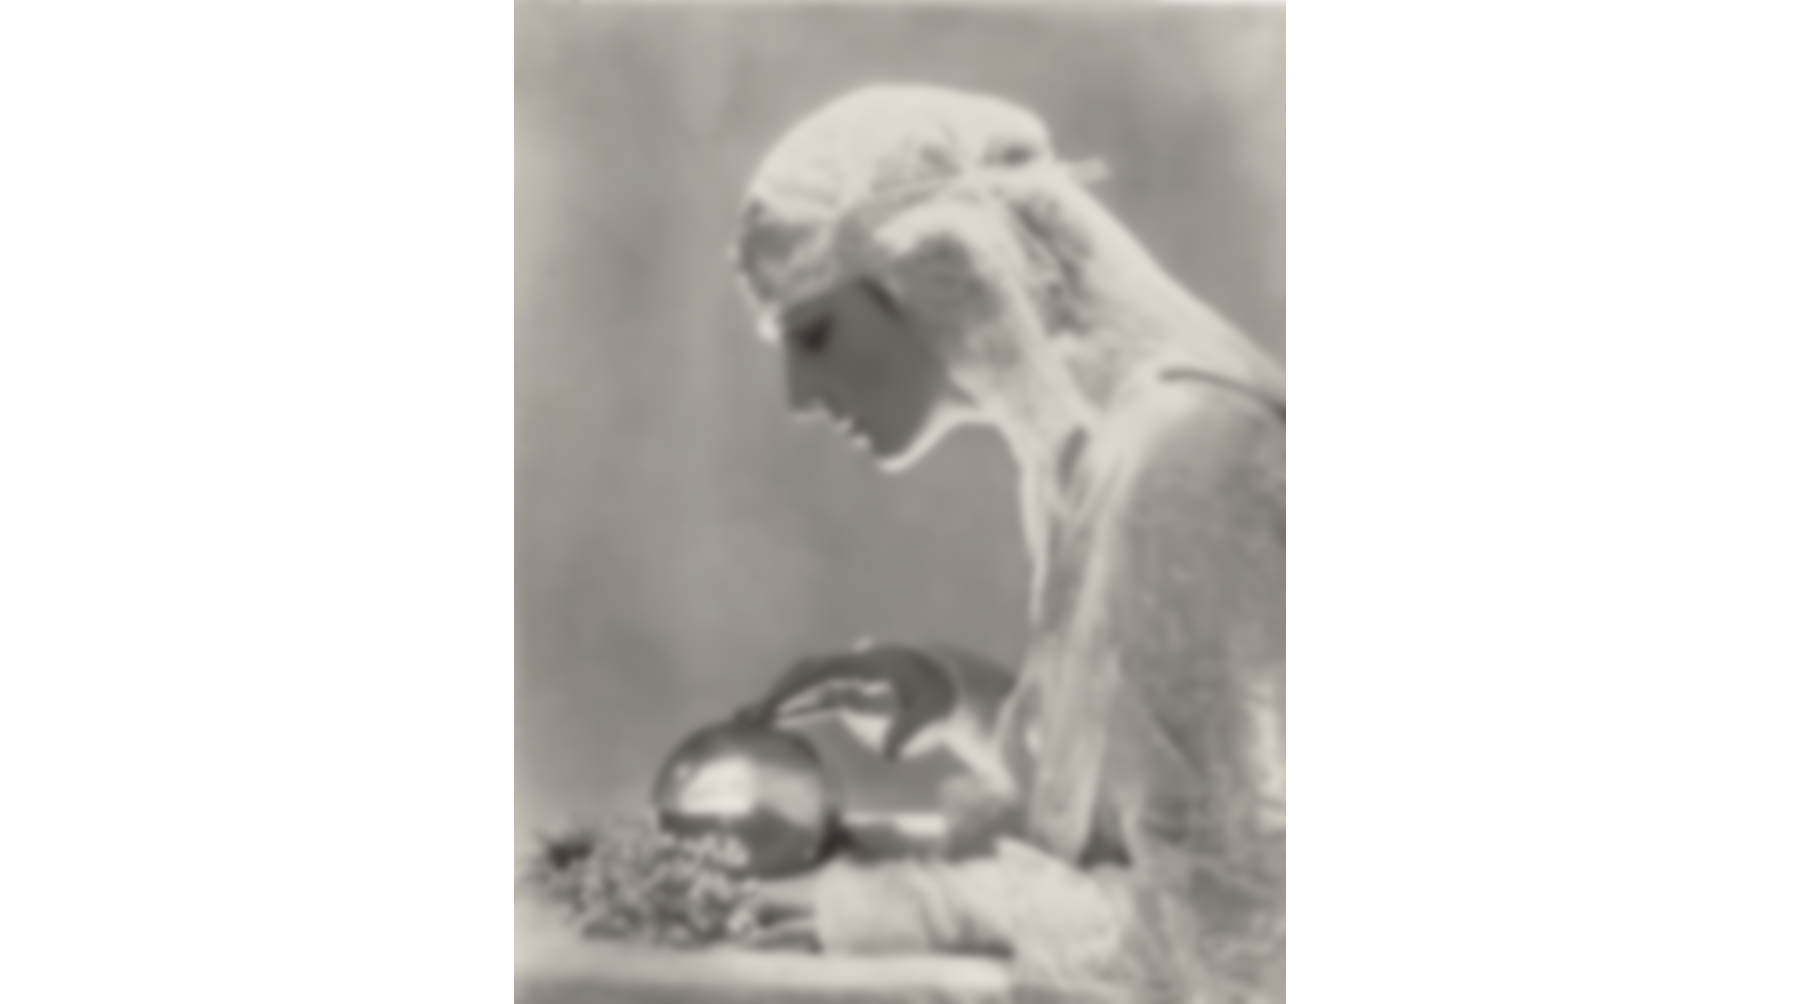
\includegraphics[width=\paperwidth]{imgs/oracle2-back.png}}
\begin{frame}
\begin{block}{Oracle}
	\begin{itemize}
		\item predict job length
		\begin{itemize}
			\item job parameters
			\item users history
		\end{itemize} \pause
		\item predict new job arrival
		\begin{itemize}
			\item users history
		\end{itemize}
	\end{itemize}
\end{block}
\end{frame}
}

\begin{frame}
	\frametitle{Measuring the schedule quality}
	\begin{itemize}
	\item users
		\begin{itemize}
			\item completion time
		\end{itemize}
\pause
	\item resource providers
		\begin{itemize}
			\item{happy users}
			\item{utilisation}
		\end{itemize}
\pause
	\item grid operator
		\begin{itemize}
			\item information
		\end{itemize}
	\end{itemize}
\end{frame}

\section{Distributed model}
\subsection{Large marketplace}

\begin{frame}
	\frametitle{Distributed scheduling}
	\pause
	\begin{itemize}
		\item execution of jobs is very localised \pause
		\item bin packing instead of job scheduling
	\end{itemize}
\end{frame}

\subsection{Multiple GRIDs}

\begin{frame}
	\frametitle{Multiple GRIDs}
	\begin{itemize}
		\item MetaCentrum and CERIT
		\item problematic establishment of cross-access policies
	\end{itemize}
\end{frame}


\section{Conclusion}
\subsection{Summary}

\begin{frame}
\frametitle{Summary}
	\begin{itemize}
		\item super computer, cluster, grid, cloud \pause
		\item job scheduling on grid \pause
		\item multi-dimensionality \pause
		\item non-clairvoyance \pause
		\item on-line scheduling \pause
		\item oracle \pause
		\item measuring quality \pause
		\item distributed scheduling
	\end{itemize}
\end{frame}

\subsection{Conclusion}

\begin{frame}
\hspace{0.7cm}

\includegraphics[width=0.2\textwidth]{filogo.pdf}
\hspace{1cm}
\begin{minipage}[b]{0.3\textwidth}

\includegraphics[width=\textwidth]{cesnet-logo-800.png}\newline

\includegraphics[width=\textwidth]{metalogo1.png}
\end{minipage}
\hspace{0.4cm}
\begin{minipage}[b]{0.3\textwidth}

\includegraphics[width=\textwidth]{cerit-sc-logo.png}
\vspace{1cm}
\end{minipage}
\end{frame}

\begin{frame}
	\frametitle{This presentation featured images from the following sources}
	BlueGene: \url{http://www.fotopedia.com/items/flickr-3334947628}\newline
	Marketplace: \url{http://www.flickr.com/photos/decade_null/2062148643/}\newline
	Oracle: \url{https://secure.flickr.com/photos/centralasian/5583102954/}
\end{frame}

\end{document}
